\documentclass[11pt]{article}
\usepackage{geometry}                % See geometry.pdf to learn the layout options. There are lots.
\geometry{letterpaper}                   % ... or a4paper or a5paper or ... 
%\geometry{landscape}                % Activate for for rotated page geometry
%\usepackage[parfill]{parskip}    % Activate to begin paragraphs with an empty line rather than an indent
\usepackage{graphicx}
\usepackage{amssymb}
\usepackage{epstopdf}
\usepackage{hyperref}
\DeclareGraphicsRule{.tif}{png}{.png}{`convert #1 `dirname #1`/`basename #1 .tif`.png}

\title{Safety Cases for Software Product Lines}
%\author{The Author}
\date{}                                           % Activate to display a given date or no date

\begin{document}
\maketitle
%
%
\section{Introduction}
%Software systems are everywhere, including safety critical domains. Software is inherently embedded into medical devices, power plant controllers, airplane controllers, drones, and soon self-driving vehicles. Safety analysis of this category of systems is an essential ingredient of the Software Development Lifecycle (SDLC). Safety cases are the most common artifacts resulting from safety analysis.
%
%Orthogonally, most of the aforementioned examples of safety critical software systems are engineered as Software Product Lines (SPLs). Variability is inherent in families of software systems. Variability can be due to different deployment environments, differences in hardware devices and peripherals, varying requirements across models of systems, and difference in performance characteristics.
%
%Variability in an SPL is usually measured in terms of the number of features in a product line. The number of possible products that can be synthesized from an SPL grows exponentially with the number of features. As a result, enumerating all possible products and performing safety analysis at the product level is intractable. 
%
%Several attempts have been made to leverage the high degree of commonality across products of an SPL to minimize the cost of product line analysis in general, and safety analysis in particular. This document explores previous attempts and fundamental questions at the crossroads of Safety Analysis and Software Product Lines.
%
\subsection{Goals}
%This document aims at:
%\begin{itemize}
%\item Surveying existing techniques
%\item Identifying gaps and pragmatic requirements that are not fulfilled by existing techniques
%\item Identifying any underlying research questions
%\end{itemize}
%
\subsection{Non-Goals} 
%
%The following are beyond the scope of this document:
%
%\begin{itemize}
%\item Coming up with new notations or techniques
%\item Empirical assessment of existing techniques
%\item Formalizing any of the discussed concepts
%\end{itemize}
%
%\subsection{Running Example}
%
%Throughout this document we use a Fuel Level Display Product Line (FLDPL) example from \cite{Gallucci_2013}. This is a simply product line safety case that extends a single product ISO26262 safety case \cite{Dardar_2014}. The diagrams in this document also come from \cite{Gallucci_2013} unless otherwise specified.
%
%\section{Existing Techniques}
%
\section{Software Product Lines (SPLs)}

\subsection{Basic Concepts}

Variability is commonplace in software systems. Managing variability across different software artifacts, and throughout the Software Development Life Cycle (SDLC) is always a challenge though. Software Product Line Engineering draws an analogy to industrial product lines, where different variants of a product are manufactured using a common set of parts and machinery. The goal of SPLs is to maximize reuse across different variants of a software product, while at the same time simplifying the extensibility and maintainability of the product line.

We start with some basic definitions, together with some simple examples illustrating them. The definitions and the object store example presented here are adapted from those in \cite{Thum}.

\begin{description}

\item[Software Product Line]
A Software Product Line (SPL) is a set of similar software products built from a common set of artifacts (e.g. design/specification models, code constructs, test cases, etc...).

\end{description}

For example, let us consider a product line of simple object stores. An object store can support the storage of a single object or multiple objects. Orthogonally, the store can provide some access control mechanism allowing only certain users to store objects. Store capacity (SingleObject vs MultiObject) and access control are just examples of possible variability points in an SPL.

\begin{description}

\item[Feature]
A feature is an externally visible property, aspect or quality of a software system.

\end{description}

In our object store SPL, SingleObject, MultiObject and access control are the 3 features within this product line.

An individual product can be generated from an SPL by selecting a set of features for that product. Not all product combinations are valid though. For example, it does not make sense for an object store to be SingleObject and MultiObject at the same time. Those two features are supposed to be mutually exclusive in our product line. This kind of constraints are captured by a \emph{Feature Model}:

\begin{description}

\item[Feature Model]
(also knows as Variability Model) is a specification of the valid combinations of features in an SPL. This is typically expressed as a boolean formula over features.

\end{description}

For example, a boolean formula expressing our mutual exclusion condition for SingleObject and MultiObject stores, together with an optional AccessControl feature, would be:

$(SingleObject \vee MultiObject) \wedge (\neg SingleObject \vee \neg MultiObject) $

\begin{description}

\item[Feature Diagram]
a hierarchical graphical representation of a Feature Model, where each non-root feature depends on its parent.

\end{description}

\begin{figure}
  \centering
    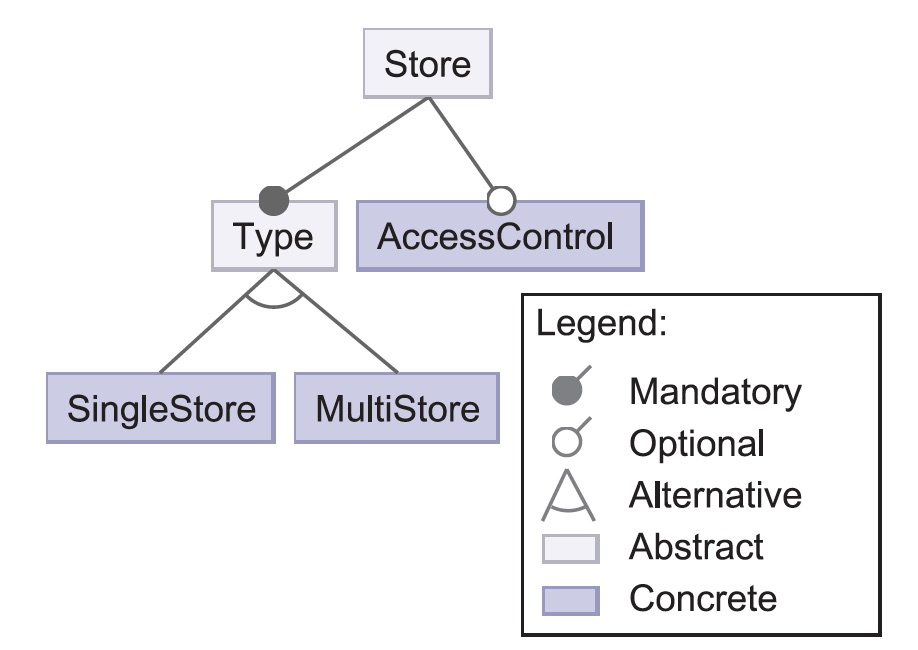
\includegraphics[width=0.75\textwidth]{FeatureDiagram}
  \caption{Feature Diagram Example}
  \label{fig:FeatureDiagram}
\end{figure}

For example, figure \ref{fig:FeatureDiagram} shows a feature diagram for our SPL.

\begin{description}

\item[Presence Condition]
A Presence Condition (PC) is a boolean formula over the set of features that does not conflict with the Feature Model.
\end{description}

For example, a product where we have the MultiObject and AccessControl features can be represented by the following PC: $ MultiObject \wedge AccessControl $

\subsection{SPL Engineering Approaches}

\subsubsection{Generative}

%In Generative Product Lines, each feature is designed and implemented separately, and then given a product configuration, a product is automatically generated out of the separate feature artifacts. Examples of Generative Product Line approaches include Feature-Oriented Programming and Aspect-Oriented Programming.
%
\subsubsection{Annotative}
%
%In Annotative Product Lines, a single set of artifacts is maintained, and feature expressions (presence conditions) are used to annotate different syntactic constructs belonging to different families of products. The most commonly used Annotative technique is C Pre-Processor (CPP) macro annotations surrounding fragments of source code.
%
\subsubsection{Delta-Oriented}
%
%In Delta-Oriented Product Lines, a base product is fully defined, and variants are defined in terms of their differences with respect to the base product. 
%
\section{Safety Cases}

\subsection{Goal Structuring Notation (GSN)}
%
%Goal Structuring Notation is used to layout logical arguments connecting safety goals to pieces of evidence satisfying them. A safety case in GSN is typically composed of 3 kinds of artifacts:
%
%\begin{figure}
%  \centering
%  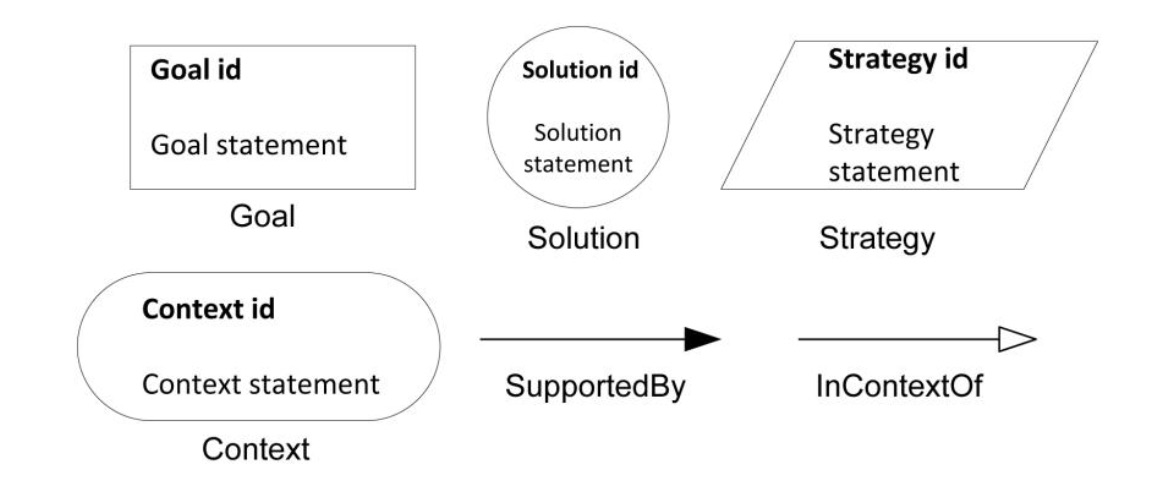
\includegraphics[width=0.75\textwidth]{gsn}
%  \caption{GSN Elements}
%\end{figure}
%
%\begin{itemize}
%\item Goals: These are the safety goals (requirements) identified as a result of hazard analysis techniques
%\item Solutions(Evidences): These are pieces of evidence that a risk/hazard is mitigated. Evidences can be test case results, formal verification outputs, or manual investigation reports
%\item Strategies: a strategy provides the logical argument connecting safety goals to their corresponding mitigating evidences
%\end{itemize}
%
%\subsubsection{Structured Assurance Case Metamodel (SACM)}
%
%SACM \cite{SACM} is an Object Management Group (OMG) standard. SACM integrates well with other OMG metamodels (e.g. UML). It provides a much richer notation compared to GSN. The notation is composed of the following metamodels:
%
%\begin{itemize}
%\item An Argumentation Meta-model
%\item An Evidence Meta-model
%\end{itemize}
%
%\section{Adding Variability}
%
%\subsection{GSN Modules and Patterns}
%
%\subsubsection{GSN Modules}
%
%Modules are a GSN extension that facilitate modularity and reuse in safety cases. GSN elements (goals, evidences and strategies) can be packages into modules, and those modules can be reused in different contexts.
%
%\begin{figure}
%  \centering
%  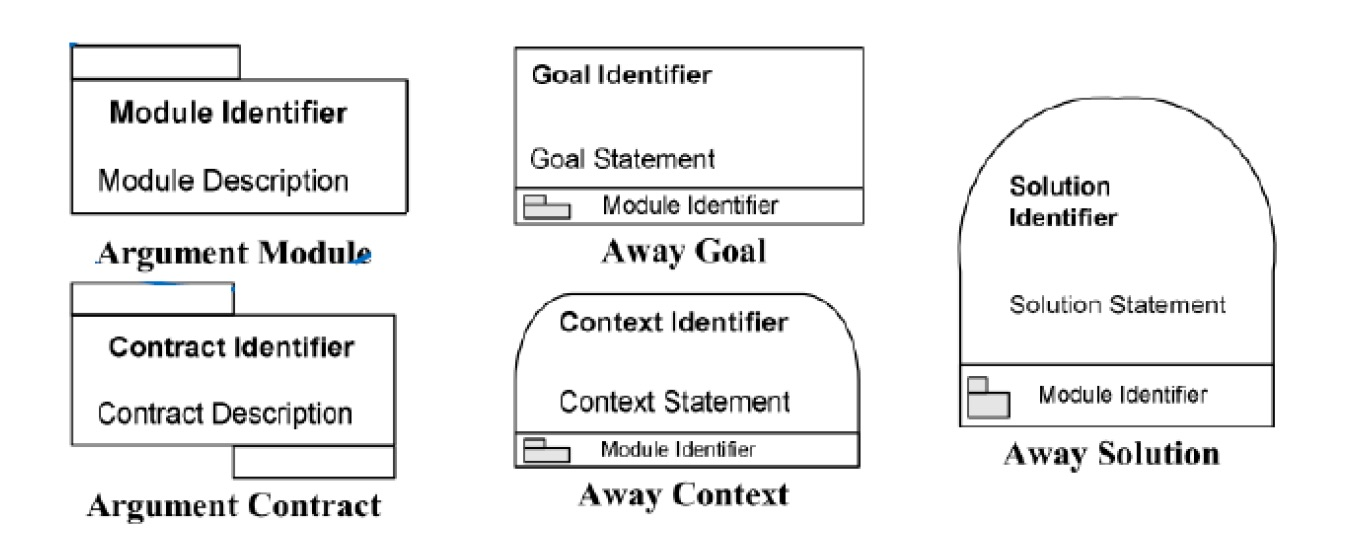
\includegraphics[width=0.75\textwidth]{gsn-modules}
%  \caption{GSN Module Constructs}
%\end{figure}
%
%\subsubsection{GSN Patterns}
%
%GSN patterns are yet another GSN extension. A GSN pattern is a parameterized GSN item. A pattern can then be instantiated by binding a parameter to a concrete value.
%
%\begin{figure}
%  \centering
%  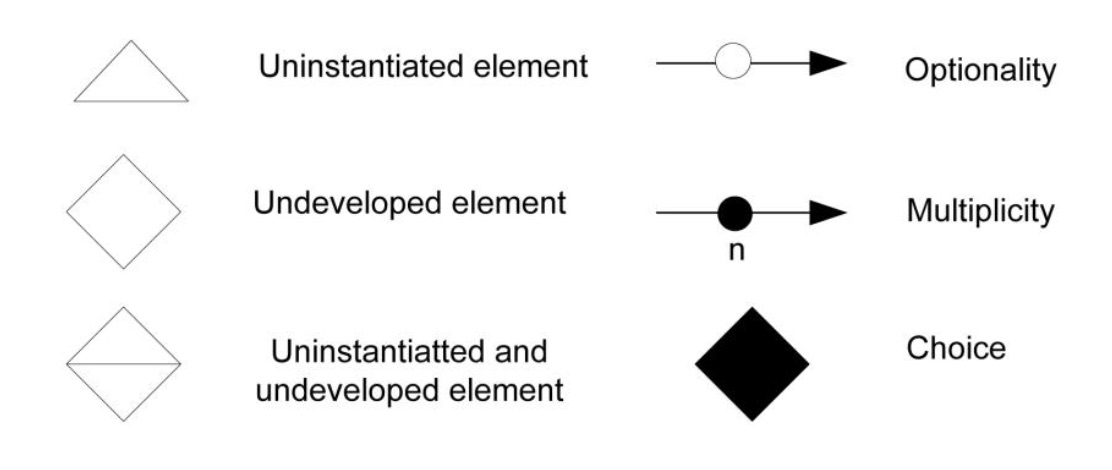
\includegraphics[width=0.75\textwidth]{gsn-patterns}
%  \caption{GSN Pattern Constructs}
%\end{figure}
%
%As an example of a GSN pattern, a generic hazard avoidance pattern would be in the context of an identified hazard, aiming at assuring that the system is safe by addressing that hazard.
%
%\begin{figure}
%  \centering
%  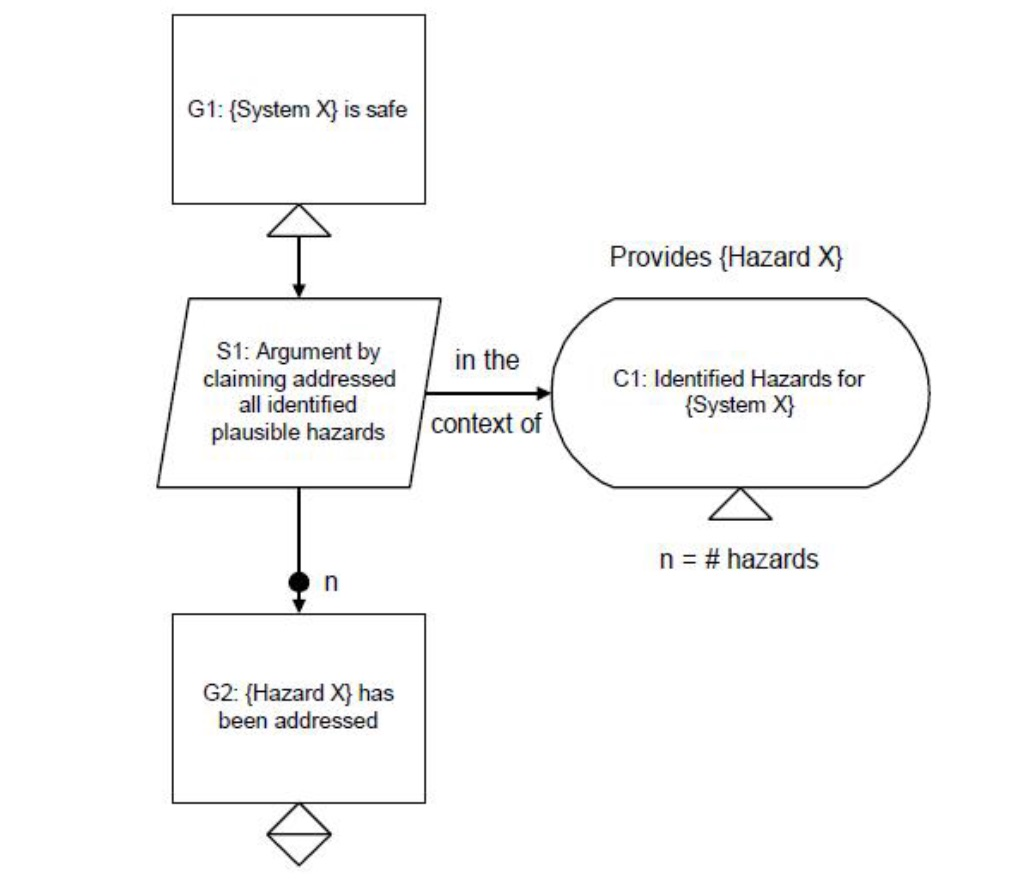
\includegraphics[width=0.75\textwidth]{gsn-pattern-example}
%  \caption{GSN Pattern Example - Hazard mitigation}
%\end{figure}
%
%\subsubsection{GSN Product Line Example}
%
%This is just a fragment of the safety case in \cite{Gallucci_2013}, demonstrating the use of GSN modules:
%
%\begin{figure}
%  \centering
%  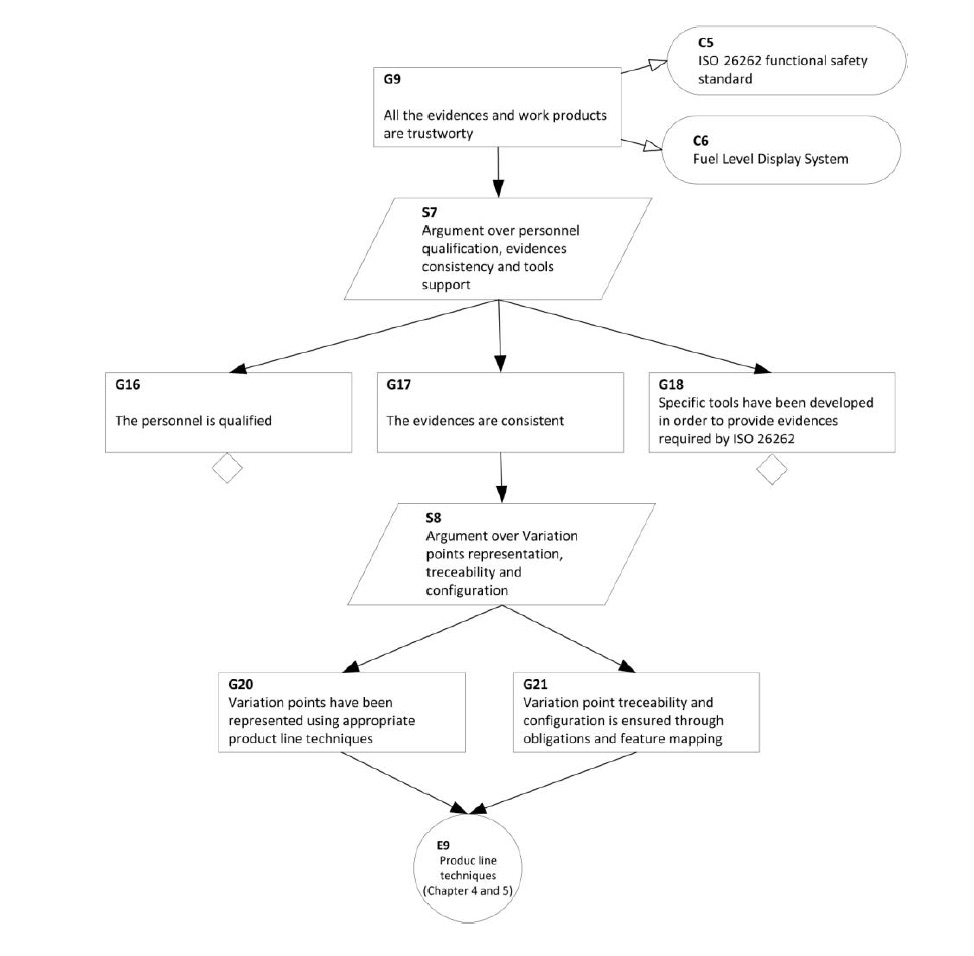
\includegraphics[width=0.75\textwidth]{safetyCase}
%  \caption{Safety Case Fragment}
%\end{figure}
%
%%3.2	Comparative Analysis
%%
%%GSN+
%%SACM?
%%GM
%%Expressivity
%%
%%
%%
%%Syntactic Conciseness
%%
%%
%%
%%Well-defined Semantics?
%%
%%
%%
%%Semantic Consistency
%%
%%
%%
%%Traceability within a single product
%%
%%
%%
%%Traceability across products
%%
%%
%%
%%
%

\subsection{Example}

\section{Discussion}
%
\subsection{Product Line Scenarios}
%
%Software Product Lines can come into existence in several ways. This section briefly outline engineering scenarios yielding Product Lines.
%
\subsubsection{Product Evolution over Time}
%
%Starting with a single product, variability might start exhibiting itself in lots of different ways. Different deployment environments, different modes of operations, minor requirement variations from different stakeholders, and varying workloads are all examples of product-level variability. Over time, the maintenance of software artifacts with too much ad-hoc variability becomes a real problem. 
%One way to manage ad-hoc variability is to evolve a single product with variability in a product line. This process usually starts with factoring out a common core (common to all variants), and variant-specific artifacts.
%
\subsubsection{Product Component Reuse}
%
%Again starting with a single component-oriented product, some components might be potentially reused in other products. Sometimes a component can be reused as is, without the need for any modification. In other cases the component might require minor modifications, resulting in a slightly different version. 
%
%This component-level variability can again evolve into a component-level Product Line. With more and more components being reused in this fashion, a component Product Line library becomes the skeleton of a Software Product Line.
%
\subsubsection{Product-Line Engineering}
%
%The previously outlined scenarios start with a single product, and with more and more variability introduced the product evolves into a product line. Sometimes on the other hand the designers of a system are aware from day one that they are building a family or products, not just one. If at design time they draw a clear boundary between a common core and a set of varying artifacts, they are actually engineering a Product Line.
%
\subsection{Product Lines and Safety Cases}
%
%Reasoning about Software Product Lines is not straightforward because of several reasons:
%
%\begin{itemize}
%
%\item The number of possible valid products of a product lines grows exponentially with the number of features. As a result, enumerating all possible valid products becomes intractable, and thus existing product-level reasoning techniques don't directly scale to product lines.
%
%\item A Feature Model is an integral part of a Product Line, and its role is to define the valid set of feature combinations. When reasoning about a Product Line, the Feature Model has to be taken into consideration to avoid including invalid products in any argument.
%
%\item Whenever an argument is made regarding a Product Line, it is essential to specify whether this argument applies to all valid products (universal quantification over products), or only to some (existential quantification). 
%
%\end{itemize}
%
\subsection{Q1: Product-Line of Safety Cases or a Safety Case of a Product Line}
%
%Safety Analysis is one example of reasoning about a software systems. Techniques like Hazard Analysis, Fault Tree Analysis and Safety Cases have been well studied and applied to software products. However, when it comes to Product Lines, those techniques do not directly scale due to the previously mentioned reasons. 
%
%In addition, one fundamental question pertains to the granularity to which Safety Analysis is performed. We can think of 2 different approaches here:
%
%\begin{itemize}
%
%\item A Safety Case of a Product Line: here safety analysis as a process is applied to a Software Product Line, resulting in a single Safety Case covering the whole Product Line.
%
%\item A Product Line of Safety Cases: since a Safety Case itself is a Software Artifact (albeit a semi-formal one at best), we can have a Product Line of Safety Cases (pretty much like Product Lines of Use Case Diagrams, Class Diagrams or Source Code artifacts). 
%
%\end{itemize}
%
\subsection{Product Line evolution impact analysis}
%
%As an SPL evolves over time (with changing requirements or more variability), existing safety cases need to evolve as well. This is essential to maintain the validity of the safety arguments. However, the safety assurance process is expensive in terms of resources and is also time consuming and labor intensive. As a result, as much of existing evidences should be reused as possible, without jeopardizing the validity of the safety arguments. Two questions are relevant here:
%
%\begin{itemize}
%
%\item Q2: As an SPL evolves, which pieces of evidence are still valid, and can be reused as is?
%
%\item Q3: Within a single piece of evidence, how much reuse can be achieved? For example, if the results of a test suite and considered a piece of evidence, how much of the test cases are common across variants and how much are variant-specific? How easy is it to draw a correspondence between features, goals/sub-goals and evidences/sub-evidences? 
%
%\end{itemize}
%
\bibliographystyle{abbrv}
\bibliography{SafetyCasesPL}

\end{document} 